\def\year{2020}\relax
%File: formatting-instruction.tex
\documentclass[letterpaper]{article} % DO NOT CHANGE THIS
\usepackage{aaai20}  % DO NOT CHANGE THIS
\usepackage{times}  % DO NOT CHANGE THIS
\usepackage{helvet} % DO NOT CHANGE THIS
\usepackage{courier}  % DO NOT CHANGE THIS
\usepackage[hyphens]{url}  % DO NOT CHANGE THIS
\usepackage{graphicx} % DO NOT CHANGE THIS
\urlstyle{rm} % DO NOT CHANGE THIS
\def\UrlFont{\rm}  % DO NOT CHANGE THIS
\usepackage{graphicx}  % DO NOT CHANGE THIS
\frenchspacing  % DO NOT CHANGE THIS
\setlength{\pdfpagewidth}{8.5in}  % DO NOT CHANGE THIS
\setlength{\pdfpageheight}{11in}  % DO NOT CHANGE THIS
%\nocopyright
%PDF Info Is REQUIRED.
% For /Author, add all authors within the parentheses, separated by commas. No accents or commands.
% For /Title, add Title in Mixed Case. No accents or commands. Retain the parentheses.
 \pdfinfo{
/Title (AAAI Press Formatting Instructions for Authors Using LaTeX -- A Guide)
/Author (AAAI Press Staff, Pater Patel Schneider, Sunil Issar, J. Scott Penberthy, George Ferguson, Hans Guesgen)
} %Leave this	
% /Title ()
% Put your actual complete title (no codes, scripts, shortcuts, or LaTeX commands) within the parentheses in mixed case
% Leave the space between \Title and the beginning parenthesis alone
% /Author ()
% Put your actual complete list of authors (no codes, scripts, shortcuts, or LaTeX commands) within the parentheses in mixed case. 
% Each author should be only by a comma. If the name contains accents, remove them. If there are any LaTeX commands, 
% remove them. 

% DISALLOWED PACKAGES
% \usepackage{authblk} -- This package is specifically forbidden
% \usepackage{balance} -- This package is specifically forbidden
% \usepackage{caption} -- This package is specifically forbidden
% \usepackage{color (if used in text)
% \usepackage{CJK} -- This package is specifically forbidden
% \usepackage{float} -- This package is specifically forbidden
% \usepackage{flushend} -- This package is specifically forbidden
% \usepackage{fontenc} -- This package is specifically forbidden
% \usepackage{fullpage} -- This package is specifically forbidden
% \usepackage{geometry} -- This package is specifically forbidden
% \usepackage{grffile} -- This package is specifically forbidden
% \usepackage{hyperref} -- This package is specifically forbidden
% \usepackage{navigator} -- This package is specifically forbidden
% (or any other package that embeds links such as navigator or hyperref)
% \indentfirst} -- This package is specifically forbidden
% \layout} -- This package is specifically forbidden
% \multicol} -- This package is specifically forbidden
% \nameref} -- This package is specifically forbidden
% \natbib} -- This package is specifically forbidden -- use the following workaround:
% \usepackage{savetrees} -- This package is specifically forbidden
% \usepackage{setspace} -- This package is specifically forbidden
% \usepackage{stfloats} -- This package is specifically forbidden
% \usepackage{tabu} -- This package is specifically forbidden
% \usepackage{titlesec} -- This package is specifically forbidden
% \usepackage{tocbibind} -- This package is specifically forbidden
% \usepackage{ulem} -- This package is specifically forbidden
% \usepackage{wrapfig} -- This package is specifically forbidden
% DISALLOWED COMMANDS
% \nocopyright -- Your paper will not be published if you use this command
% \addtolength -- This command may not be used
% \balance -- This command may not be used
% \baselinestretch -- Your paper will not be published if you use this command
% \clearpage -- No page breaks of any kind may be used for the final version of your paper
% \columnsep -- This command may not be used
% \newpage -- No page breaks of any kind may be used for the final version of your paper
% \pagebreak -- No page breaks of any kind may be used for the final version of your paperr
% \pagestyle -- This command may not be used
% \tiny -- This is not an acceptable font size.
% \vspace{- -- No negative value may be used in proximity of a caption, figure, table, section, subsection, subsubsection, or reference
% \vskip{- -- No negative value may be used to alter spacing above or below a caption, figure, table, section, subsection, subsubsection, or reference

\setcounter{secnumdepth}{0} %May be changed to 1 or 2 if section numbers are desired.

% The file aaai20.sty is the style file for AAAI Press 
% proceedings, working notes, and technical reports.
%
\setlength\titlebox{2.5in} % If your paper contains an overfull \vbox too high warning at the beginning of the document, use this
% command to correct it. You may not alter the value below 2.5 in
%\title{AAAI Press Formatting Instructions \\for Authors Using \LaTeX{} --- A Guide }
\title{ Outer Dictionary LSTM: An Efficient Network For Named Entity Recognition }
%Your title must be in mixed case, not sentence case. 
% That means all verbs (including short verbs like be, is, using,and go), 
% nouns, adverbs, adjectives should be capitalized, including both words in hyphenated terms, while
% articles, conjunctions, and prepositions are lower case unless they
% directly follow a colon or long dash
%\author{Written by AAAI Press Staff\textsuperscript{\rm 1}\thanks{Primarily Mike Hamilton of the Live Oak Press, LLC, with help from the AAAI Publications Committee}\\ \Large \textbf{AAAI Style Contributions by
%Pater Patel Schneider,} \\ \Large \textbf{Sunil Issar, J. Scott Penberthy, George Ferguson, Hans Guesgen}\\ % All authors must be in the same font size and format. Use \Large and \textbf to achieve this result when breaking a line
%\textsuperscript{\rm 1}Association for the Advancement of Artificial Intelligence\\ %If you have multiple authors and multiple affiliations
% use superscripts in text and roman font to identify them. For example, Sunil Issar,\textsuperscript{\rm 2} J. Scott Penberthy\textsuperscript{\rm 3} George Ferguson,\textsuperscript{\rm 4} Hans Guesgen\textsuperscript{\rm 5}. Note that the comma should be placed BEFORE the superscript for optimum readability
%2275 East Bayshore Road, Suite 160\\
%Palo Alto, California 94303\\
%publications20@aaai.org % email address must be in roman text type, not monospace or sans serif
%}
\author{Junxiang Ge, Qi Zhang, Haizhou Zhao\\ 
AI Research Department, Sogou \\
Beijing, China}
 \begin{document}

\maketitle

\begin{abstract}
%AAAI creates proceedings, working notes, and technical reports directly from electronic source furnished by the authors. To ensure that all papers in the publication have a uniform appearance, authors must adhere to the following instructions. 
With the risen use of AI application, we need to understand some specific type of message from user's query. Named Entity Recognition(NER) is a basic task for that use. Gazzete is very useful when doing NER, howerver, most of the current method use iit in word embedding format, which will bring out the case, we need to retrain model when the word in gazzete is greatly changed. In this paper, we propose a conception, called Outer Dictionary LSTM (OD-LSTM), which means to use the outer type info of gazzete for each word, without using the specific word. Experiments shows it useful when doing NER task, and acheive a great improvement on task with which gazzete is heavily depended on.
\end{abstract}

%\noindent Congratulations on having a paper selected for inclusion in an AAAI Press proceedings or technical report! This document details the requirements necessary to get your accepted paper published using PDF\LaTeX{}. If you are using Microsoft Word, instructions are provided in a different document. AAAI Press does not support any other formatting software. 
%
%The instructions herein are provided as a general guide for experienced \LaTeX{} users. If you do not know how to use \LaTeX{}, please obtain assistance locally. AAAI cannot provide you with support and the accompanying style files are \textbf{not} guaranteed to work. If the results you obtain are not in accordance with the specifications you received, you must correct your source file to achieve the correct result. 
%
%These instructions are generic. Consequently, they do not include specific dates, page charges, and so forth. Please consult your specific written conference instructions for details regarding your submission. Please review the entire document for specific instructions that might apply to your particular situation. All authors must comply with the following:
%
%\begin{itemize}
%\item You must use the 2020 AAAI Press \LaTeX{} style file and the aaai.bst bibliography style file, which are located in the 2020 AAAI Author Kit (aaai20.sty and aaai.bst).
%\item You must complete, sign, and return by the deadline the AAAI copyright form (unless directed by AAAI Press to use the AAAI Distribution License instead).
%\item You must read and format your paper source and PDF according to the formatting instructions for authors.
%\item You must submit your electronic files and abstract using our electronic submission form \textbf{on time.}
%\item You must pay any required page or formatting charges to AAAI Press so that they are received by the deadline.
%\item You must check your paper before submitting it, ensuring that it compiles without error, and complies with the guidelines found in the AAAI Author Kit.
%\end{itemize}

\section{Introduction}
Named Entity Recognition (NER) is a base task when doing many Natural Language Processing (NLP) tasks. Usually, we need to extract mainly information from users' sentences to help us understand their meanings, and then use the extracted information to do further process. For example, in weather domain, we may need to extract \textbf{date and position} to help us understand when and where the user is asked towards the weather; in music type service, we may need to track \textbf{singer, song, style } entities to suit user's command; for many commom use, we need \textbf{person, location, organization} message to understand a sentence.

To accomplish this task, many method has been explored.  Convolution Neural Network (CNN) is used in Image Classification (Krizhevsky, Sutskever and Geoffrey 2012), and then proved also powerful in Text Classification (Kim 2014). CNN is also useful in NER tasks, whether to capture character-level features (Chiu and Nichols 2016; Ma and Hovy 2016; Peters et al. 2017), or to do word-level sequence labelling (Santos, Xiang, and Zhou 2015; Strubell et al. 2017). To learn the correlation between words in sentence, Recurrent Neural Network (RNN) (Sutskever, Vinyals and Le 2014) and Long Short-Term Memory (LSTM)  (Sak, Senior and Beaufays 2014) are proposed, and they achieve great success on machine translation area and so on. They are then used in NER tasks and achieve significant improvement (Chiu and Nichols 2016; Ma and Hovy 2016; Peters et al. 2017). These structures can be use in different situations (Yang, Liang, and Zhang 2018). As the depth of Nerual Network (NN) usually improve the final performance, more and more complicated method has been proposed in recent years. Transformer structure (Vaswani et al. 2017) and its derivative methods, like OpenAI GPT (Radford et al. 2018), BERT (Devlin et al. 2018), XLNet (Yang et al. 2019), make innovative attempt to NN structures. 

Among these years, many method focus on base layer of NN structure, usually the embedding input layer, and then directly use it to do NLP tasks (Peters et al. 2018; Radford et al. 2018; Devlin et al. 2018; Yang et al. 2019). Though will it make improvement, it usually pays a long time to train the model. But in these way, it tell us that embedding input can directly infect the result of NLP tasks. 

There exists a little difference between English NER tasks and Chinese NER tasks. In Chinsese or other hieroglyphics language, character means a single word; and word is a character phrase which has length longer than one. In English or other letter base language, character means a single letter, and word is a composition of letters. English word is composed by characters, for which character level CNN can help improve NER tasks (Huang et al. 2015; Chiu and Nichols 2016; Ma and Hovy 2016; Peters et al. 2017; Yang, Liang, and Zhang 2018); but that can not be use in Chinese NER tasks, which is hieroglyphics. For this reason, Chinese NER tasks is usually done by word baseline or character baseline structure. Word baseline structure refer to using word segmentor to split sentence into word tokens and then use their word vector (Peng and Dredez 2015; Peng and Dredez 2016); while character structure simply treat each sentence into combination of single Chinese character, and then using character embedding to do NLP tasks (Zhang and Yang 2018; Gui et al. 2019). In these methods, it seems useful when using word embedding within character baseline structure, or the oppisite. 

Most of state-of-the-art NER methods uses Conditional Random Fields (CRF) (Lafferty, McCallum, and Pereira 2011) to decode the sequence labelling result. CRF can work even without any NN cells. Hand-writing trait can sometimes already achieve high performance (Finkel, Grenager, and Manning 2005; Okazaki 2007). 

In some situations, word backgound knowledge, namely dictionary (the same meaning as lexicon and gazette), is neccessary to do NER jobs. For example, in music service case, “You Raise Me Up'' would be treated more likely as a chat information rather than a song, unless the model is given that knowledge (see in Figure \ref{fig1}). Most of the state-of-the-art methods using word embedding to complete these task. But it then gives two problems: 

\begin{itemize}
\item Out Of Vacabulary (OOV) problem. As for \textbf{song} entity in music service, word embedding size will be too large; and sometimes will the length of song be too long to make word vector. 
\item Retrain problem. When the content of dictionary changes abundantly, the trained model would have poor performance doing the same jobs. Still use the \textbf{song} entity as an example, the dictionary would be changed monthly or even daily, thus we need to retrain our model synchronously. 
\end{itemize}

Faced with this problem, we proposed a new conception, called Outer Dictionary (OD) models, which means using the dictionary's outer trait, without using its specific content. For example, we use the word type `` song ``, rather than a specific song name, to help model understand the outer information. In these way, word embedding is no longer needed for Chinese NER task. Exprement result show that in gazzete depended-on task, OD model gives the best result among state-of-the-art method. And when the content of dictionary changed, the model can synchronously update its result without retraining.

\begin{figure}[t]
\centering
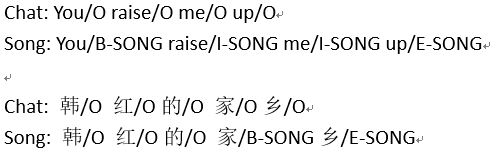
\includegraphics[width=0.9\columnwidth]{gazzete_is_needed} % Reduce the figure size so that it is slightly narrower than the column. Don't use precise values for figure width.This setup will avoid overfull boxes. 
\caption{In certain NER situation, dictionary info is neccessary, as cases showed in figure. With knowing the certain name is a song, we tend to denote the word as a song rather a common sentence.}
\label{fig1}
\end{figure}

\subsection{Contributions}

In summary, we make these contributions:

\begin{itemize}
\item We proposed a new conception: Outer Dictionary (OD) model, which is used to update the content of dictionary without retraining the model.
\item In order to realize OD model, we explored Tag Embedding LSTM (TE-LSTM), using the word type, rather the word itself, to improve the performance of NER tasks.
\item Experiment result shows our model gives significant improvements on gazzete depended-on tasks among state-of-the-art models.
\item We release the music service dataset, which we use in our paper, for further scientific research.
\end{itemize}

\section{Related Work}
Success of BERT (Devlin et al. 2018) and XLNet (Yang et al. 2019) show that word embedding is important and useful for many upper NLP tasks. More useful information is there in the vector, more efficiently the model would work. To a great degree, embedding layer decides the performance. Same conclusion can be made from a lot of NER models, as for character level message, word level message, position message, handwriting message and so on. Especially in some specific NER task, like music service, gazzete is heavilly depended on to make better performance. 

Most of the recent models use gazette as word embedding input, or its string format, to give the model related message. Lattice LSTM (Zhang and Yang 2018) use the embedding as additional input to character baseline LSTM, which can give the model more sentence information. Lexivon Rethinking CNN (Gui et al. 2019), corparate the word embedding vector to correlated CNN layer, and the coflict word segment could be learned by rethinking. Stanford NER (Finkel, Grenager, and Manning 2005) can use the gazette information, as string format, in CRF model.

However, in some pratical use, the content of the gazette will change greatly and constantly. In this way, most of the recent model need to be retrained after every abundantly change of gazette. To solve this problem, we need to construct a model which can still be used after such change. We then came out with the OD models, and use TE-LSTM to realize these model. As a result, with no more word embedding is needed, and model needed only to be trained once.  What we need is the word tag information to help the model better understand user's intention.

\section{Outer Dictionary LSTM}

In this chapter, we illustrate the model we use to realize the OD model. We use the character baseline model for Chinese NER task,  inspired by the results of Lattice LSTM (Zhang and Yang 2018) and Lexicon Rething CNN (Gui et al. 2019). In order to better understand the model, we make a appointment that: In Chinsese or other hieroglyphics language, character means a single word; and word is a character phrase which has length longer than one. In English or other letter base language, character means a single letter, and a word is a composition of letters; then a phrase is composited of a set of words. For Chinese NER jobs, only character embedding will we use, and no more word embedding is needed, for we hold the following opinions towards these jobs:

\begin{itemize}
\item Common characters in hieroglyphics language, can be exhaustive,  especially for Chinese, because there are no more than 100, 000 characters in simplified Chinese. 
\item Words in hieroglyphics language, will be uncountable, because there are still many new words or pharases are still created every day. Thus, OOV error can not be avoided in these case.
\end{itemize}

Thus, in Chinese NER jobs, we denote a sentence as a composition of many characters: $s = (c_1, c_2, ..., c_n) $ as the base input to model.

\subsection{Character-Base LSTM}

We use character embedding lookup table to turn character id to vector:

\begin{equation}
a_i = e_c(c_i) \label{char_embedding}
\end{equation}

Usually a dropout layer is connected with the embedding output, which is proved useful in NER jobs (Ma and Hovy 2016). After that, bi-directional LSTM (Bi-LSTM), the most common structure used in NER tasks, is applied to learn the character connection within the sentence. We use the hidden vector for LSTM output, that is, for input: $x = (a_1, a_2, ..., a_n) $,  we get output: $h = (h_1, h_2, ..., h_n)$, where $h_i$ is the concatenation of forward ($\overrightarrow{h_i}$) and backward ($\overleftarrow{h_i}$) LSTM hidden vector:

\begin{equation}
h_i = [\overrightarrow{h_i};\overleftarrow{h_i}] \label{lstm_out}
\end{equation}

\subsection{Tag Embedding Model}

As case show in Figure \ref{fig1}, we need to use dictionary for certain NER tasks. However, the constant variation of dictionary may cause constant retrain problem. Therefore, we may not use the specific word in each dictionary, instead, only the outer information will be used, which is called Outer Dictionary (OD) model. Here, we implement our OD model using Tag Embedding (TE), which uses the tag embedding of the dictionary. Cause we use LSTM structure to utilize tag embedding info, we called our model  TE-LSTM.

Specifically, we do this by two step: 

a)  Match sentence with the word in dictionary using certain outer model method.

b)  Turn match result into embedding information, used as the input of LSTM.

\textbf{Match Policy}. In this part, we need to match all the word in given dictionary occured in current sentence. We impletement this by using Aho-Corasick Automation Algorithm (Aho and Corasick 1975). In summary, we complete a KMP (Knuth, Morris, and Pratt 1977) + Trie Tree (Briandais 1959) algorithm to accomplish this task. In methematical, given sentence $s = (c_1, c_2, ..., c_n) $, and a dictionary $d_i$, which is composed of word set $D_i=\{w_1, w_2, ..., w_V\}$. We denote the result of match policy as:

\begin{equation}
r_{d_i} = [ (f_1, b_1), (f_2 , b_2), ..., (f_k, b_k) ] \label{match_result}
\end{equation}

Here, $f_i$ and $b_i$ denote the front and back position of each match word. Let $W_{f_i,b_i}$ represent the substring of sentence $s$ with the rank $[f_i, b_i]$, then each $(f_i, b_i)$ tuple forms a word in $D_i$. Parameter $k$ means the total number of such word matched in $d_i$, which is uncertain.

\textbf{Tag Embedding Sceme}. After match policy is fullfilled, we need to turn that result into vector so that it can be understood by model. Cause the result of match policy is denoted as position, we can simply use it to get a new sequence form from original sentence. With dictionary $d_i$ and a matched word position rank range $[f_i, b_i]$, the original sentence can be written as: $ s = (c_1, c_2, ..., c_{f_i - 1}, c_{f_i}, ..., c_{b_i}, c_{b_i + 1}, ..., c_n) $, we perform this function to turn it into a new sequence:

\begin{equation}
rf(s, i, d_i, f_i, b_i) = \left \{
\begin{array}{rl}
' O ' ,& 0 < i < f_i \ or \ b_i < i <= n; \\
ts(s, i, d_i) ,& f_i <= i <= b_i;
\end{array}
\right.
\label{tag_scheme}
\end{equation}

where $ts(s, i)$ means a tag scheme function, here, we choose IOBES scheme for it is proved better than IOB1 and IOB2 tag scheme in result by previous works (Ma and Hovy 2016), and the same conclusion is proved by our experement result emprically. 

Here, we need to emphasis the fact that: the dictionary here need not to be the same with the result tag species. As an illustration, to extract \textbf{name} entities, we can use dictionary \textbf{first name} and dictionary \textbf{last name} to do this transformation.

Since there will be one or more matched word for one dictionary, in order to fix the matched word of $d_i$ in certain position, we choose $w$ words from result list. And them choose the best $w$ results from the matched list, in our experiment, here we use the word length, the longer, the best. Then with dictionary $(d_1, d_2, ..., d_m)$, the tag embedding sequence can be denoted as:

\begin{equation}
ft(s) = \left[
\begin{array}{rl}
rf(s, d_1, f_1, b_1), & \\
rf(s, d_1, f_2, b_2), & \\
...,  &\\
rf(s, d_1, f_w, b_w); &\\
...;  &\\
rf(s, d_m, f_1, b_1), &\\
rf(s, d_m, f_2, b_2), &\\
..., &\\
rf(s, d_m, f_w, b_w)]
\end{array}
\right]
\label{final_tag_sequence}
\end{equation}

\subsection{Loss and Training}
pass

\section{Experiments}

pass

\section{Conclusion}

pass

\section{ Acknowledgments}
Especially grateful to Can Cui for denoting the music ner data, to Jindou Wu for advice on data processing of CCKS 2018 music dataset.

\section{References}

\smallskip \noindent
Krizhevsky, A.; Sutskever, I.; and Geoffrey E. H. 2012. ImageNet Classification with Deep Convolutional Neural Networks. In Proceedings of  Advances in Neural Information Processing Systems 25 (NIPS 2012).

\smallskip \noindent
Kim, Y. 2014. Convolutional Neural Networks for Sentence Classification. arXiv:1408.5882.

\smallskip \noindent
Sutskever, I.; Vinyals, O.; and Le, Q.V. 2014. Sequence to Sequence Learning with Neural Networks. In Proceedings of Advances in Neural Information Processing Systems 27 (NIPS 2014).

\smallskip \noindent
Sak, H.; Senior, A.; and Beaufays, F. 2014. Long Short-Term Memory Based Recurrent Neural Network Architectures for Large Vocabulary Speech Recognition. arXiv:1402.1128.

\smallskip \noindent 
Collobert, R.; Weston, J.; Bottou, L.; Karlen, M.; Kavukcuoglu, K.; and Kuksa, P. 2011. Natural Language Processing (Almost) from Scratch. Journal of Machine Learning Research 12 (2011) 2493-2537. 

\smallskip \noindent
Santos. C. N.; Xiang, B.; and Zhou, B. 2015. Classifying Relations by Ranking with Convolutional Neural Networks. arXiv:1504.06580. 

\smallskip \noindent
Strubell, E.; Verga, P.; Belanger, D.; and McCallum, A. 2017. Fast and Accurate Entity Recognition with Iterated Dilated Convolutions. arXiv:1702.02098. 

\smallskip \noindent
Peters, M. E.; Ammar, W.; Bhagavatula, C.; and Power. R.  2017. Semi-supervised sequence tagging with bidirectional language models. arXiv:1705.00108.

\smallskip \noindent 
Peters, M. E.; Neumann, M.; Iyyer, M.; Gardner, M.; Clark, C.; Lee, K.; and Zettlemoyer, L. 2018. Deep contextualized word representations. arXiv:1802.05365. 

\smallskip \noindent
Ma, X.; and Hovy, E. 2016. End-to-end Sequence Labeling via Bi-directional LSTM-CNNs-CRF. arXiv:1603.01354. 

\smallskip \noindent
Yang, J.; Liang, S.; and Zhang, Y. 2018. Design Challenges and Misconceptions in Neural Sequence Labeling. arXiv:1806.04470. 

\smallskip \noindent
Vaswani, A.; Shazeer, N.; Parmar, N.; Uszkoreit, J.; Jones, L.; Gomez, A. N.; Kaiser, L.; and Polosukhin, I. 2017. Attention Is All You Need. arXiv:1706.03762. 

\smallskip \noindent
Radford, A.; Narasimhan, K.; Salimans, T.; and Sutskever, I. 2018. Improving Language Understanding by Generative Pre-Training. Technical report, Open AI.

\smallskip \noindent
Devlin, J.; Chang, M.; Lee, K.; and Toutanova, K. 2018. BERT: Pre-training of Deep Bidirectional Transformers for Language Understanding. arXiv:1810.04805.

\smallskip \noindent
Yang, Z.; Dai, Z.; Yang, Y.; Carbonell, J.; Salakhutdinov, R.; and Le, Q. V. 2019. XLNet: Generalized Autoregressive Pretraining for Language Understanding. arXiv:1906.08237.

\smallskip \noindent
Sang, E. F.; and Meulder, F. D. 2003. Introduction to the CoNLL-2003 Shared Task: Language-Independent Named Entity Recognition. arXiv:cs/0306050. 

\smallskip \noindent
Chiu, J. P.C.; and Nichols, E. 2016. Named Entity Recognition with Bidirectional LSTM-CNNs. Transactions of the Association for Computational Linguistics, Volume 4, 2016, p.357-370. 

\smallskip \noindent
Huang, Z.; Xu, W.; and Yu, K. 2015. Bidirectional LSTM-CRF Models for Sequence Tagging. arXiv:1508.01991. 

\smallskip \noindent
Peng, N.; and Dredze, M. 2016. Improving Named Entity Recognition for Chinese Social Media with Word Segmentation Representation Learning. arXiv:1603.00786. 

\smallskip \noindent
Chen, Q.; Zhuo, Z.; and Wang, W. 2019. BERT for Joint Intent Classification and Slot Filling. arXiv:1902.10909. 

\smallskip \noindent
Zhang, Y.; and Yang, J. 2018. Chinese NER Using Lattice LSTM. arXiv:1805.02023. 

\smallskip \noindent
Gui, T.; Ma, R.; Zhang, Q.; Zhao, L.; Jiang, Y.; and Huang, Y. 2019. CNN-Based Chinese NER with Lexicon Rethinking. In Proceedings of the International Joint Conference on Artificial Intelligence 2019 (IJCAI 2019). 

\smallskip \noindent
Lafferty, J.; McCallum, A.; and Pereira, F. 2001. Conditional Random Fields: Probabilistic Models for Segmenting and Labeling Sequence Data. In Proceedings of the 18th International Conference on Machine Learning 2001 (ICML 2001), pages 282-289.

\smallskip \noindent
Socher, R.; Manning, C. D.; and Andrew Y. Ng. 2010. Learning Continuous Phrase Representations and Syntactic Parsing with Recursive Neural Networks. In Proceedings of the NIPS-2010 Deep Learning and Unsupervised Feature Learning Workshop. 

\smallskip \noindent
Finkel, J. R.; Grenager, T.; and Manning, C. 2005. Incorporating non-local information into information extraction systems by Gibbs sampling. In Proceedings of the 43nd Annual Meeting of the Association for Computational Linguistics (ACL 2005), pp. 363-370. 

\smallskip \noindent
Okazaki, N. 2007. CRFsuite: a fast implementation of Conditional Random Fields (CRFs). URL http://www. chokkan. org/software/crfsuite. 

\smallskip \noindent
Peng, N.; and Dredze, M. 2015. Named Entity Recognition for Chinese Social Media with Jointly Trained Embeddings. In Proceedings of the 2015 Conference on Empirical Methods in Natural Language Processing (EMNLP). 

\smallskip \noindent
Mikolov, T.; Chen, K.; Corrado, G.; and Dean, J. 2013. Efficient Estimation of Word Representations in Vector Space. In Proceedings of Workshop at ICLR. 

\smallskip \noindent
Mikolov, T.; Sutskever, I.; Chen, K.; Corrado, G.; and Dean, J. 2013. Distributed Representations of Words and Phrases and their Compositionality. In Proceedings of NIPS. 

\smallskip \noindent
Mikolov, T.; Yih, W.; and Zweig, G. 2013. Linguistic Regularities in Continuous Space Word Representations. In Proceedings of NAACL HLT. 

\smallskip \noindent
Pennington, J.; Socher, R.; and Manning, C.D. 2014. GloVe: Global Vectors for Word Representation. In Proceedings of the 2014 Conference on Empirical Methods in Natural Language Processing (EMNLP), pages 1532–1543. 

\smallskip \noindent
Mikolov, T.; Grave, E.; Bojanowski, P.; Puhrsch, C.; and Joulin, A. 2017. Advances in Pre-Training Distributed Word Representations. arXiv:1712.09405. 

\smallskip \noindent
Aho, A. V.; and Corasick, M. J. 1975. Efficient string matching: An aid to bibliographic search. Communications of the ACM. June 1975, 18 (6): 333–340.

\smallskip \noindent
Knuth, D.; Morris, J. H.; and Pratt, V. 1977. Fast pattern matching in strings. SIAM Journal on Computing. 6 (2): 323–350. 

\smallskip \noindent
Briandais, D. L. R. 1959. File searching using variable length keys. Proc. Western J. Computer Conf. pp. 295–298. 

\end{document}
